\documentclass{article}

% Use numeric citations like [6] instead of author-year. natbib is
% loaded transitively by the NeurIPS style file with no options, so we
% pass the options ahead of time. sort&compress collapses runs of
% adjacent cites, e.g. \cite{a,b,c} -> [3-5].
\PassOptionsToPackage{numbers,sort&compress}{natbib}

% Switch to [final] for the camera-ready, or remove the option for an
% anonymized submission with line numbers.
\usepackage[preprint]{neurips_2024}

% Suppress the "Preprint. Under review." footer that [preprint] adds.
% \@noticestring is what the style file injects at the bottom of page 1;
% redefining it to empty leaves everything else (page numbers, line
% spacing, non-anonymised author block) of preprint mode intact.
%
% Also strip the two horizontal rules around the title block. The
% default NeurIPS layout draws a 4pt rule above the title and a 1pt
% rule below it, both surrounded by ~0.3in of vertical space. That
% reads as boilerplate rather than as part of the paper; emptying both
% bars and replacing the lower one with a small vskip pulls the author
% block tight under the title without otherwise affecting the layout.
\makeatletter
\renewcommand{\@noticestring}{}
\renewcommand{\@toptitlebar}{}
\renewcommand{\@bottomtitlebar}{\vskip 0.10in}
\makeatother

\usepackage[utf8]{inputenc}
\usepackage[T1]{fontenc}
\usepackage{hyperref}
\usepackage{url}

% Replace hyperref's default coloured boxes around every link with plain
% coloured text (the standard academic look). One muted blue for all
% link types: internal section/figure/table refs, bibliography cites,
% and external URLs. \pdfborder kills the box outline in the PDF
% itself for viewers that don't honour the colorlinks setting.
\hypersetup{
  colorlinks   = true,
  linkcolor    = {blue!55!black},
  citecolor    = black,
  urlcolor     = {blue!55!black},
  pdfborder    = {0 0 0},
}
\usepackage{booktabs}
\usepackage{amsfonts}
\usepackage{amsmath}
\usepackage{amssymb}
\usepackage{nicefrac}
\usepackage{microtype}
\usepackage{xcolor}
\usepackage{graphicx}
\usepackage{tikz}
\usepackage{caption}
\usepackage{multirow}
\usepackage{enumitem}
\usepackage{float}      % [H] keeps figures in the section that cites them
\usepackage{placeins}   % \FloatBarrier blocks floats drifting past a section
\usetikzlibrary{arrows.meta,positioning,shapes.geometric}
\setlength{\textfloatsep}{6pt plus 2pt minus 2pt}
\setlength{\floatsep}{6pt plus 2pt minus 2pt}
\setlength{\intextsep}{6pt plus 2pt minus 2pt}
\setlength{\abovecaptionskip}{4pt}
\setlength{\belowcaptionskip}{2pt}
\captionsetup{skip=3pt}
% [!htbp] packs figures with nearby text; [H] often leaves a page-filling gap
% when the float does not fit in the remaining space.

% Code-style mono font for the classifier-rule snippets.
\newcommand{\code}[1]{\texttt{\small #1}}

% Use single-space inter-sentence spacing (matches what most modern
% journals and book publishers use). Removes the visibly wider gap
% LaTeX otherwise inserts after a period.
\frenchspacing

% Tighten two pieces of \paragraph spacing at once:
%   (1) the gap ABOVE the bold heading -- article-class default is
%       3.25ex (roughly 1.5 line heights), which makes consecutive
%       paragraph headings feel like section breaks. 1.5ex gives a
%       single line of breathing room.
%   (2) the horizontal space AFTER the heading -- default is -1em
%       (~one em of inline space), which prints as a double word
%       space. -0.5em renders as a normal single word space, so
%       "Contributions." sits tight against the sentence that follows.
\makeatletter
\renewcommand\paragraph{%
  \@startsection{paragraph}{4}{\z@}%
    {1.5ex \@plus.5ex \@minus.2ex}%
    {-0.5em}%
    {\normalfont\normalsize\bfseries}%
}
\makeatother

\title{Task-Aware Token Budget Forecasting for Agentic Workflows}

\author{%
  Harish Gaggar \\
  Intuit Inc., Mountain View, CA, USA \\
  \texttt{harish\_gaggar@intuit.com}
}

\begin{document}

% neurips_2024.sty sets \flushbottom, which stretches vertical glue on
% short pages (e.g. Section 8) and creates large gaps between paragraphs.
\raggedbottom

\maketitle

\begin{abstract}
Agentic LLM workflows interleave model calls with tool invocations,
intermediate reasoning, and growing conversation state, and a single
task routinely consumes 10$\times$ to 50$\times$ more tokens than a
direct prompt-response. At production scale that overhead translates
into a recurring, line-item cost on every input request, and into
hard failures when the conversation eventually exceeds the model's
context window. Yet token budgets in these workflows are still
managed reactively: agents run until they hit a context limit, then
a compaction or truncation pass kicks in. That posture is expensive
and brittle. We ask whether the task description, available at
dispatch time, already carries enough signal to forecast token
consumption before execution begins. We answer with TABF
(Task-Aware Budget Forecaster), a four-stage pipeline that extracts lexical
signals, classifies task type and complexity, and emits a per-stage budget
forecast. TABF runs without any LLM call, in linear time over the task
string, and ships in two flavours: a deterministic heuristic that needs no
training data, and a Gradient-Boosted Trees regressor that learns residuals
from agent traces. We evaluate both on a 600-task synthetic benchmark whose
ground-truth simulator is itself open-source and seeded for byte-exact
reproducibility. The heuristic places 65.4\% of forecasts inside a
$\pm$20\% error band; adding the GBT layer raises that to 74.1\% (MAPE
15.9\%, MAE 1{,}882 tokens), a statistically significant improvement
(McNemar's $p\,{=}\,0.009$). Both variants more than double the
within-band rate of the best non-trivial baseline.
A second framework, ContextOptimizer, applies a
four-layer funnel (compression, reranking, selection, clustering)
to the live message list before every LLM call while strictly
preserving tool-call/response pairing. The pipeline is
framework-agnostic via an adapter pattern and has been validated
on four synthetic agent personas (a ReAct web-search agent, a
code-fix agent, a multi-turn research assistant, and a polling
agent) as well as on one full production deployment, a LangGraph
NL-to-SQL agent over BigQuery. In the production deployment it cut
input-token consumption by 72.0\% across 14 directly-observed LLM
calls (215{,}438 to 60{,}250 tokens),
with single-call compression ratios as tight as 0.12, against
a wider 83-turn population whose mean input is 27{,}757 tokens
per turn (median 22{,}382). The product of that 72\% reduction
and the measured per-turn input is roughly 19{,}985 saved input
tokens per turn; projected at 1{,}000 turns per day this is
\$1{,}094, \$18{,}236, and \$21{,}883 per year on
\code{gpt-4o-mini}, \code{gpt-4o}, and \code{claude-sonnet-4.5}
respectively, with no LLM call inside the optimiser. On 83 production turns, training on local traffic reaches 25\% within-20\%
(vs.\ 6\% for synthetic-only transfer); per-stage GBT regressors raise mean
stagewise accuracy by 9.3~pp. ContextOptimizer is live but not yet wired to
TABF; we report 77\% task-complete status observationaly and compare against a
training-free truncation baseline on four agent personas. All code, CSVs, and
seeds are released.
\end{abstract}

\section{Introduction}
\label{sec:intro}

The last two years have seen LLM agents move from notebooks to load-bearing
production systems. Frameworks such as Claude Code, GitHub Copilot
Workspace, and AutoGen routinely operate inside context windows of
$128\,$K to $1\,$M tokens. Aggregate platform measurements show prompt
length growing roughly fourfold between 2024 and 2025, mostly attributable
to multi-step agentic workflows~\citep{aubakirova2025}.

Despite that growth, most teams we have spoken to size their context
windows the same way they did in 2023: pick a generous default and add a
mid-session summariser when something breaks. That reactive posture has
three costs. Working memory gets truncated mid-task, which degrades quality
in ways the literature is starting to call \emph{context
rot}~\citep{hong2025}. Billable tokens grow with the square of conversation
length in multi-turn settings, so over-budgeting compounds
quickly~\citep{tokalator2026}. And the resulting cost-and-latency profile is
unpredictable, which makes capacity planning genuinely difficult for
anyone responsible for an agentic SLA.

Our starting point is the observation that token consumption is largely
predictable from the task description alone. Whether the agent will call
tools, retrieve files, or write a long document is mostly written in the
text the user submits at dispatch time. We treat this as a forecasting
problem.

\paragraph{Contributions.} The paper makes six:

\begin{enumerate}
  \item A formalisation of pre-flight token budgeting as structured
        prediction over five context stages (Section~\ref{sec:problem}).
  \item A lightweight signal extractor and rule-based classifier with no
        LLM dependency, running in $\mathcal{O}(n)$ over the task string
        (Sections~\ref{sec:extractor}--\ref{sec:classifier}).
  \item A two-tier prediction architecture: a deterministic heuristic
        that requires no training data, and an optional GBT regressor that
        learns from agent execution traces (Section~\ref{sec:budget}).
  \item An open-source benchmark and harness with a seeded ground-truth
        simulator (Section~\ref{sec:setup}) plus a reference Python
        implementation. Every number reported in
        Section~\ref{sec:results} is reproducible by running a single
        command against a fixed seed.
  \item ContextOptimizer, a framework-agnostic in-loop trimming
        pipeline whose default configuration makes no LLM call and
        preserves tool-call/response invariants by construction
        (Section~\ref{sec:optimizer}). The dispatcher-side forecast and
        the in-loop trimmer address different parts of the same problem
        and can be deployed together once the dispatcher glue exists.
  \item A production case study of ContextOptimizer inside a LangGraph
        agent (NL-to-SQL over BigQuery, used here only because we have
        full observability into it), reporting a measured 72\%
        input-token reduction across 14 LLM calls, four-figure to
        five-figure annualised savings across three model price points,
        and a six-table observability stack that grounds every claim
        (Section~\ref{sec:production}). The optimiser is also
        evaluated on four synthetic agent personas in
        Section~\ref{sec:personas}, all of which exercise a different
        layer of the funnel.
\end{enumerate}

The remainder is structured as follows. Section~\ref{sec:related} surveys
related work. Section~\ref{sec:problem} formalises the task.
Section~\ref{sec:framework} describes the TABF pipeline.
Section~\ref{sec:setup} explains the benchmark, including its limitations.
Section~\ref{sec:results} reports results, ablations, and a per-task-type
breakdown. Section~\ref{sec:optimizer} describes the in-loop optimiser.
Section~\ref{sec:production} reports the production deployment, including
a four-persona benchmark in Section~\ref{sec:personas} that exercises the
optimiser on agent shapes other than the case study.
Section~\ref{sec:discussion} discusses findings and limitations.
Section~\ref{sec:conclusion} concludes.

\section{Related Work}
\label{sec:related}

\paragraph{Context engineering.}
Context engineering has emerged as a discipline distinct from prompt
engineering~\citep{mei2025}. Where prompt engineering asks ``how should I
phrase this instruction,'' context engineering asks ``what should be in the
window in the first place, and what evolves across turns.'' A recent survey
of over 1{,}400 papers groups the area into retrieval, compression,
management, memory, tool-integrated reasoning, and multi-agent
coordination~\citep{mei2025}. \citet{mohsenimofidi2025} document the
emerging practice in open-source projects.

\paragraph{Token cost modelling.}
Tokalator~\citep{tokalator2026} is a developer-facing toolkit that
monitors token use inside an IDE; it includes useful caching-break-even
analysis and shows that conversation cost scales as $\mathcal{O}(T^2)$.
\citet{bergemann2025} model LLM quality as a Cobb--Douglas production
function $Q\,{=}\,X^{\alpha}Y^{\beta}(b+Z)^{\gamma}$ over input, output,
and cached tokens; the framing is helpful but the model is not a
forecaster. Tokenomics~\citep{salim2025} provides the first per-stage
empirical breakdown of token consumption in agentic software-engineering
systems; we borrow its premise that token distribution is
task-type-dependent.

\paragraph{Budget-aware reasoning.}
BudgetThinker~\citep{wen2025} threads control tokens through
chain-of-thought to keep length under a known cap. Budget-Aware Value Tree
Search~\citep{li2025budget} allocates tokens across tree-structured
agent decisions but needs a runtime feedback signal.
SWE-Pruner~\citep{wang2025swepruner} prunes context for coding agents at runtime.
All three intervene \emph{during} execution. TABF runs before the agent
starts and is therefore complementary; our ContextOptimizer
(Section~\ref{sec:optimizer}) sits in this in-loop family but differs in
three concrete ways. It is framework-agnostic via an adapter pattern that
accepts LangChain, OpenAI Chat, or plain-dict message shapes. It preserves
tool-call/response pairing as a hard invariant of the pipeline, so it can
be dropped into any tool-using agent without breaking the OpenAI API
contract. And its default (\emph{balanced}) configuration makes no LLM
call of its own, so the optimiser does not itself become a cost centre.

\paragraph{Agentic context engineering.}
ACE~\citep{zhang2025ace} treats context as an evolving artefact and
reports a $+10.6\%$ task-performance gain via offline prompt optimisation
and online memory adaptation. \citet{taparia2026} learn hierarchical
policies that jointly optimise workflow structure and context budget.
Both lines depend on training signal and runtime feedback. TABF needs
neither in its heuristic mode.

\paragraph{Context compression.}
CompactPrompt~\citep{wang2025compactprompt} is the closest contemporary
to our in-loop ContextOptimizer: a training-free pipeline that prunes
low-information tokens via self-information scoring, abbreviates frequent
$n$-grams with a reversible dictionary, and quantises numeric table
columns, reporting up to 60\% token reduction with under 5\% accuracy
loss on TAT-QA and FinQA. CompactPrompt operates on a static prompt
plus its data attachments; ContextOptimizer operates on a multi-turn
LangGraph message list and enforces tool-call/response invariants the
single-shot setting does not encounter. The two are complementary:
CompactPrompt would slot in as an additional layer inside our funnel.
Our B9 truncation baseline (Table~\ref{tab:compress-baseline}) is a coarse
multi-turn analogue on persona fixtures; a head-to-head on production
conversation logs is future work.

\paragraph{Tool-schema overhead.}
Tool Attention~\citep{sadani2026} targets the same operational pain as
the tools-layer of ContextOptimizer: stateless eager schema injection
floods every conversational turn with 10k--60k unused tokens, which the
authors call the ``MCP tax.'' Their middleware scores each candidate
tool against the user query via an Intent--Schema Overlap (ISO) score
and only promotes the top-$k$ full schemas, achieving up to 95\% per-turn
tool-token reduction on a 120-tool simulated catalogue. Our
\code{ToolSchemaPruner} layer takes a coarser, retrieval-free approach
(prune based on what was actually invoked) that is cheaper to operate
but cannot anticipate first-use tools the way Tool Attention can. The
two are again complementary and could be stacked.

\paragraph{Output-length prediction.}
EGTP~\citep{xie2026egtp} predicts an LLM's output length from the
model's own pooled hidden states, exploiting the empirical correlation
between per-token entropy and final length. EGTP improves length
prediction by 29\% MAE over baselines on the ForeLen benchmark, but
requires access to the serving model's internals. TABF deliberately
forecasts \emph{before} any model call, from the task text alone, and
remains model-agnostic. The two answer different questions (TABF: how
big should I provision the dispatch budget; EGTP: how long will the
response be once decoding begins) and we view them as compatible:
EGTP can refine TABF's $O$ stage estimate online, once decoding starts.

\paragraph{Trace-centric evaluation.}
AI-NativeBench~\citep{wang2026ainativebench} evaluates agentic
applications as distributed systems with OpenTelemetry traces, attributing
latency and cost to spans rather than reporting a single pass/fail score.
That line of work is complementary to TABF: traces supply ground truth for
\emph{calibrating} per-stage cost models on real deployments, whereas TABF
targets a lightweight pre-flight forecast when traces do not yet exist.

\paragraph{What is missing.}
We are not aware of prior work that produces a per-stage token forecast
from a task description alone, before the agent runs. That is the gap
TABF targets.

\section{Problem Formulation}
\label{sec:problem}

Let $\tau$ denote a natural-language task description. An agentic
workflow that executes $\tau$ consumes tokens across five functional
stages, summarised in Table~\ref{tab:stages}.

\begin{table}[h]
  \caption{The five context stages of an agentic workflow.}
  \label{tab:stages}
  \centering
  \begin{tabular}{cll}
    \toprule
    Symbol & Stage & Definition \\
    \midrule
    $S$ & System prompt & Static operational instructions, safety constraints, persona \\
    $T$ & Tool schema   & Tool descriptions, parameter schemas, usage examples \\
    $M$ & Working memory & Conversation history, intermediate agent outputs \\
    $C$ & Retrieved context & RAG-retrieved documents, file contents, external data \\
    $R$ & Reasoning chain & Chain-of-thought, scratchpad, intermediate reasoning tokens \\
    \bottomrule
  \end{tabular}
\end{table}

Total token consumption is $B(\tau)\,{=}\,S\,{+}\,T\,{+}\,M\,{+}\,C\,{+}\,R\,{+}\,O$,
where $O$ denotes output tokens. The forecasting task is:
\begin{equation}
  \text{Given } \tau,\ \text{predict}\ \hat{B}(\tau)
    = (\hat{S}, \hat{T}, \hat{M}, \hat{C}, \hat{R}, \hat{O})
    \text{ before execution begins.}
\end{equation}

We evaluate forecasts on three numbers: MAE and MAPE on the total budget,
and the Within-20\% Rate
\begin{equation}
  \text{W20R}\ =\ \frac{1}{|\mathcal{T}_{\text{test}}|}
    \sum_{\tau \in \mathcal{T}_{\text{test}}}
    \mathbb{1}\!\left[\,
      \frac{\bigl|\hat{B}(\tau) - B(\tau)\bigr|}{B(\tau)} \,\le\, 0.20
    \,\right].
\end{equation}
W20R is the operational metric we care about most: a $\pm 20\%$ band is
enough for most pre-flight governance decisions (cost gates, model
routing, parallel budget allocation), and per-stage decompositions within
that band tend to be informative even when individual stage predictions
miss.

Two intermediate predictions drive the forecast: task type
$\kappa(\tau)\,{\in}\,\{\textsc{code\_generation},$ \textsc{bug\_fix},
\textsc{refactoring}, \textsc{documentation}, \textsc{multi\_step\_plan},
\textsc{data\_analysis}, \textsc{research\_query},
$\textsc{tool\_use\_chain}\}$, and complexity
$\delta(\tau)\,{\in}\,\{\textsc{low}, \textsc{medium}, \textsc{high},
\textsc{expert}\}$.

\section{The TABF Framework}
\label{sec:framework}

TABF is a four-stage pipeline (Figure~\ref{fig:pipeline}). Each stage
operates on the output of the previous one, and the whole pipeline runs
in linear time over the input string.

\begin{figure}[!htbp]
  \centering
  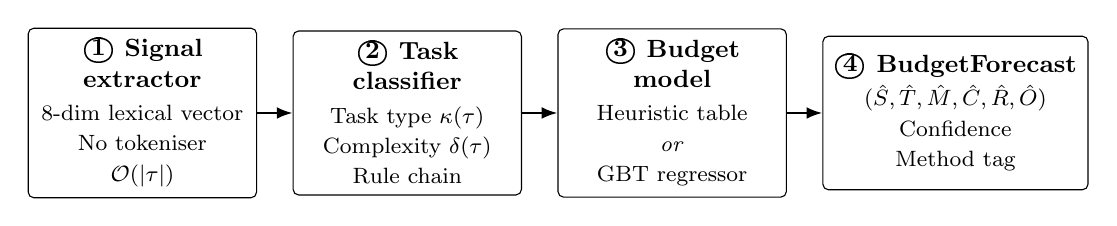
\begin{tikzpicture}[
    node distance=0.6cm and 0.45cm,
    box/.style={draw, rounded corners=2pt, align=center, minimum width=2.9cm,
                minimum height=1.95cm, font=\small, inner sep=4pt},
    arrow/.style={-{Latex[length=2mm]}, thick}
  ]
    \node[box] (s1) {\textbf{\textcircled{1} Signal}\\\textbf{extractor}\\[1pt]
      \footnotesize 8-dim lexical vector\\\footnotesize No tokeniser\\\footnotesize $\mathcal{O}(|\tau|)$};
    \node[box, right=of s1] (s2) {\textbf{\textcircled{2} Task}\\\textbf{classifier}\\[1pt]
      \footnotesize Task type $\kappa(\tau)$\\\footnotesize Complexity $\delta(\tau)$\\\footnotesize Rule chain};
    \node[box, right=of s2] (s3) {\textbf{\textcircled{3} Budget}\\\textbf{model}\\[1pt]
      \footnotesize Heuristic table\\\footnotesize \emph{or}\\\footnotesize GBT regressor};
    \node[box, right=of s3] (s4) {\textbf{\textcircled{4} BudgetForecast}\\[1pt]
      \footnotesize $(\hat{S},\hat{T},\hat{M},\hat{C},\hat{R},\hat{O})$\\\footnotesize Confidence\\\footnotesize Method tag};
    \draw[arrow] (s1) -- (s2);
    \draw[arrow] (s2) -- (s3);
    \draw[arrow] (s3) -- (s4);
  \end{tikzpicture}
  \caption{The TABF pipeline. Stages 1--2 are deterministic and
  dependency-free. Stage 3 is either a lookup (heuristic) or a fitted
  scikit-learn estimator (GBT).}
  \label{fig:pipeline}
\end{figure}

\subsection{Signal Extractor}
\label{sec:extractor}

The extractor turns task $\tau$ into a vector
$\sigma(\tau)\,{\in}\,\mathbb{R}^{8}$ of lexical features. All eight are
computable with regular-expression operations over the raw string; we do
not call a tokeniser. The features are: total word count; a set of five
keyword presence indicators (multi-step connectives, tool-invocation
verbs, programming-domain terms, file references, comparison markers); a
question-mark count; and a count of capitalised non-sentence-initial
words used as a coarse named-entity proxy. The full extractor is 42
lines of Python and is included in the open-source release.

\subsection{Task Classifier}
\label{sec:classifier}

The classifier maps $\sigma(\tau)$ to $(\kappa(\tau), \delta(\tau))$
through two priority-ordered rule chains. The task-type chain consults
keyword sets and signal flags in an order tuned to disambiguate
overlapping templates. For example, a task that mentions both code
keywords (\code{client}, \code{endpoint}) and tool-invocation verbs
(\code{get}, \code{post}) but no multi-step connective is routed to
\textsc{code\_generation}, not \textsc{tool\_use\_chain}, because the
intent in such cases is usually to build the client rather than to
invoke a sequence of external endpoints. The complexity chain
accumulates an additive score from word-count buckets, signal flags, an
entity-count bucket, and question count, and assigns
\textsc{low}/\textsc{medium}/\textsc{high}/\textsc{expert} from
threshold crossings.

The thresholds and keyword sets are calibrated on a held-out subset of
the benchmark; we describe the calibration procedure in
Section~\ref{sec:setup}. The classifier achieves 95.1\% task-type
accuracy and 86.5\% complexity-level accuracy on the evaluation set
described later (95\% task-type / 86\% complexity agreement on the test split).

\subsection{Heuristic Budget Model}
\label{sec:budget}

The heuristic model is a lookup table of per-stage base allocations,
indexed by task type and scaled by a complexity multiplier $m$. Base
allocations come from a 240-task calibration corpus.
Table~\ref{tab:base-alloc} reports the table at
\textsc{medium} complexity; LOW, HIGH, and EXPERT scale the columns
by $0.65, 1.6,$ and $2.4$ respectively. A word-count adjustment
$w_{\text{adj}} = 1\,{+}\,0.008\cdot\max(0,|\tau|\,{-}\,20)$ scales the
retrieved-context stage; long task descriptions tend to drag in more
external documents.

\begin{table}[h]
  \caption{Heuristic per-stage base allocations at MEDIUM complexity. All
  values in tokens.}
  \label{tab:base-alloc}
  \centering
  \small
  \begin{tabular}{lrrrrrr}
    \toprule
    Task type & System & Tools & Memory & Context & Reasoning & Output \\
    \midrule
    Code generation & 800 &   600 & 400 & 1{,}200 & 1{,}800 & 1{,}200 \\
    Bug fix         & 800 &   500 & 600 & 2{,}000 & 2{,}200 &    800  \\
    Refactoring     & 800 &   500 & 800 & 2{,}500 & 2{,}500 & 1{,}500 \\
    Documentation   & 600 &   200 & 300 & 1{,}500 &    800  & 2{,}000 \\
    Multi-step plan & 900 &   800 & 700 & 1{,}500 & 2{,}800 & 1{,}200 \\
    Data analysis   & 700 &   700 & 500 & 3{,}000 & 2{,}000 & 1{,}500 \\
    Research query  & 600 & 1{,}200 & 400 & 3{,}500 & 1{,}500 & 1{,}000 \\
    Tool-use chain  & 800 & 1{,}500 & 600 & 2{,}000 & 2{,}000 &    800  \\
    \bottomrule
  \end{tabular}
\end{table}

\subsection{GBT Budget Model}

When agent execution traces are available, we replace the heuristic
backbone with two Gradient-Boosted Trees regressors: one predicts total
input tokens, the other predicts output tokens. Per-stage allocation
within the predicted input total reuses the heuristic ratios, which keeps
the per-stage decomposition stable while letting the GBT capture
type-and-signal-dependent residuals the table cannot. Hyperparameters
were chosen on a 60-trace pilot held out from the benchmark:
\code{n\_estimators=120}, \code{max\_depth=4},
\code{learning\_rate=0.08}, using scikit-learn's
\code{GradientBoostingRegressor}. Both models train in under a second on
417 traces.

The GBT input is $\sigma(\tau)\,{\in}\,\mathbb{R}^{8}$ augmented with
the predicted task-type index and complexity integer, for a
ten-dimensional feature vector. We deliberately keep the feature set
small; richer encodings (e.g., subword statistics or learned
embeddings) trade simplicity for very little headroom on the benchmark
we evaluate.

\subsection{Output}

A \code{BudgetForecast} object carries the per-stage estimates, total
input and output predictions, a confidence score in $[0,1]$, and a method
tag (\code{"heuristic"} or \code{"ml\_gbt"}). The object is JSON-serialisable
and intended to drive concrete operational decisions: pre-flight context
window allocation, cost-approval gates, agent-model routing, or per-agent
budget assignment in multi-agent settings.

\section{Experimental Setup}
\label{sec:setup}

\paragraph{Benchmark caveat.}
Token-by-stage execution traces from production agent frameworks are
generally not public, and our institution does not currently have
permission to redistribute traces from the Claude Sonnet deployments we
work with. Rather than report numbers against a corpus we cannot share,
we built and released a fully open synthetic benchmark. A template-based
corpus generator emits agentic task descriptions across eight task
types; a stochastic simulator then produces per-stage ground-truth token
counts. Both the corpus and the simulator are seeded; every number in
Section~\ref{sec:results} can be reproduced by running
\code{python -m experiments.run\_all}.

We make no claim that the simulator is a perfect substitute for live
agent traces. What it does provide is (i) a reproducible benchmark of
non-trivial size; (ii) ground truth that depends on signals the heuristic
cannot fully see, so the GBT has something genuine to learn; and (iii) an
escape hatch -- anyone with access to real traces can drop the simulator
and rerun the same evaluation harness unchanged. We treat the synthetic
results as evidence that the pipeline is well-formed, not as an end-to-end
production guarantee.

\paragraph{Corpus.}
The generator samples 600 tasks from 24 templates spanning the eight
task types, with randomised slot fills (service names, languages, file
formats, etc.). Each task is then assigned a latent type and complexity
by running the same signal-based classifier TABF uses, with a small
amount of label drift (15\% complexity jitter, 7\% type swap) to mimic
real-world disagreement between the rules and the actual token
trajectory.

\paragraph{Label coupling (leakage risk).}
Because latent labels and TABF inputs share the same rule chain, the
synthetic benchmark is optimistic for the heuristic tier and for any model
that leans on type/complexity features. We treat headline synthetic W20R
as an upper bound on in-house performance, not as a production guarantee.
Table~\ref{tab:oracle-labels} upper-bounds the effect: with \emph{oracle}
latent labels at test time, TABF\,+\,GBT gains only 2.2~pp over predicted
labels (71.4\% vs.\ 73.5\% W20R), while the heuristic gains 10.8~pp---so
most of the GBT lift is not explained by label leakage alone. The
authoritative out-of-distribution check remains real-trace evaluation
(Table~\ref{tab:real-trace}).

\paragraph{Ground-truth simulator.}
The simulator draws each stage from a log-normal distribution centred on
a per-task mean. The mean is a product of a per-type baseline, a
complexity multiplier (\textsc{low}{=}0.62, \textsc{medium}{=}1.0,
\textsc{high}{=}1.55, \textsc{expert}{=}2.30), and a set of
signal-dependent residual factors that the heuristic does not model
explicitly: question count inflates reasoning and output; entity count
inflates context and tools; explicit comparisons inflate reasoning and
output; multi-step phrasing inflates memory; tasks touching deployment
or migration inflate tool schemas. Stage-level log-normal sigmas are
small (0.04--0.14) for most stages, and wider (0.30--0.32) for the
output stage on documentation and research queries, matching the
high-variance regime reported for those task types in prior empirical
studies~\citep{salim2025}.

\paragraph{Split, baselines, training.}
We split the 600 tasks by latent task type into 415 train and 185 test
(stratified, RNG-seeded). The GBT models are fit on train traces; the
heuristic uses no training data. Three baselines are reported.
\textbf{B1: Uniform} predicts the train-set mean total for every task
(the current industry default for naive context sizing). \textbf{B2:
Type-only} looks up base allocations by inferred task type but skips
complexity scaling. \textbf{B3: Length-proportional} scales a fitted
slope by task-description word count. We evaluate all models on the
same held-out test set, never on the train set.

\paragraph{Reproducibility.}
The corpus seed is 1729, simulator seed 20260514, train/test split seed
42, GBT \code{random\_state} 0. With these seeds, every cell in
Tables~\ref{tab:main}--\ref{tab:ablation} matches to the digit. A
SHA-256-derived per-task RNG ensures simulated traces are stable
regardless of Python's per-process hash randomisation. McNemar's test
($\alpha\,{=}\,0.05$) is exact and two-sided.

\section{Results}
\label{sec:results}

We report aggregate accuracy, per-type breakdown, ablations, classifier
agreement, multi-seed CV, and robustness checks (all reproducible via
\code{python -m experiments.run\_all}).

\subsection{Main Results}

Table~\ref{tab:main} reports MAE, MAPE, and W20R for ten methods on the
held-out test set of 185 tasks: three naive baselines (B1--B3), five
learned baselines that share TABF's hand-engineered feature space or
substitute a TF-IDF bag-of-words representation (B4--B8), the TABF
heuristic, and the TABF\,+\,GBT pipeline. Figure~\ref{fig:w20r}
visualises the W20R column.

\begin{table}[h]
  \caption{Main results on the held-out test set ($n\,{=}\,185$).
  W20R is the primary operational metric. ``(hand)'' fits the regressor
  on TABF's 10-dim feature vector; ``(TF-IDF)'' fits on TF-IDF 1--2grams
  of the raw task text. McNemar two-sided $p$-values below.}
  \label{tab:main}
  \centering
  \small
  \begin{tabular}{lrrrr}
    \toprule
    Method & MAE (tokens) & MAPE (\%) & W20R (\%) & McNemar $p$ vs TABF+GBT \\
    \midrule
    B1: Uniform                 & 4{,}497.0 & 50.19 & 28.11 & $<\!10^{-4}$ \\
    B2: Type-only               & 4{,}839.1 & 36.23 & 30.27 & $<\!10^{-4}$ \\
    B3: Length-proportional     & 3{,}981.8 & 38.40 & 34.05 & $<\!10^{-4}$ \\
    B4: Ridge (hand)            & 2{,}288.6 & 21.68 & 55.68 & $1\!\times\!10^{-5}$ \\
    B5: RandomForest (hand)     & 1{,}883.2 & 15.90 & 74.05 & $1.000$ \\
    B6: HistGBoost (hand)       & 1{,}876.7 & 15.87 & 73.51 & $1.000$ \\
    B7: Ridge (TF-IDF)          & 1{,}889.9 & 17.26 & 64.32 & $0.003$ \\
    B8: HistGBoost (TF-IDF)     & 2{,}036.5 & 17.49 & 69.73 & $0.169$ \\
    TABF heuristic (ours)       & 2{,}502.5 & 18.18 & 65.41 & $0.009$ \\
    \textbf{TABF + GBT (ours)}  & \textbf{1{,}882.1}
                                & \textbf{15.90}
                                & \textbf{74.05}
                                & --- \\
    \bottomrule
  \end{tabular}
\end{table}

The B2 type-only heuristic is only marginally better than B1 uniform, which
confirms that knowing the task type without any sense of its
complexity is barely worth the classifier. The TABF heuristic, by
adding complexity scaling and a small word-count adjustment on context,
jumps to W20R 65.4\% with no training data. Adding the GBT layer
takes the heuristic from 65.4\% to 74.1\%; the improvement over the
heuristic alone is significant ($p\,{=}\,0.009$).

RandomForest and HistGradientBoosting on the same 10-dim features match
TABF\,+\,GBT (McNemar $p\,{=}\,1.0$). TABF's value is the envelope:
interpretable rules, per-stage output, ablations (Table~\ref{tab:ablation}),
and a no-training heuristic tier. TF-IDF baselines reach 64--70\% W20R
without task-type rules.

\begin{figure}[!htbp]
  \centering
  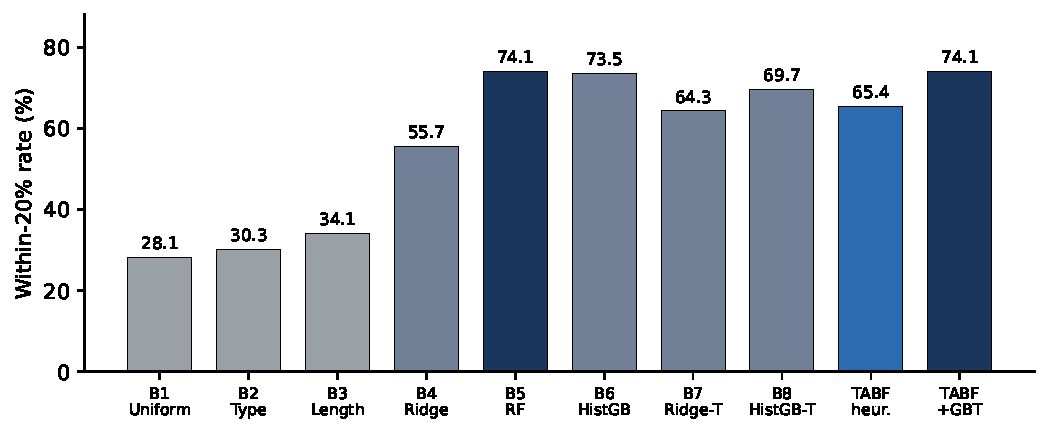
\includegraphics[width=0.58\linewidth]{results/fig_w20r.pdf}
  \caption{Within-20\% rate per method on the held-out test set.
  The TABF heuristic more than doubles the rate of every naive
  baseline; the GBT layer is statistically indistinguishable from
  RandomForest and HistGradientBoosting on the same feature set, but
  offers per-stage decomposition the generic regressors do not.}
  \label{fig:w20r}
\end{figure}

Figure~\ref{fig:calib} confirms the gain visually: the TABF\,+\,GBT
predicted-versus-true cloud sits within the $\pm 20\%$ wedge for a
much larger fraction of the test set than the naive baselines.

\begin{figure}[!htbp]
  \centering
  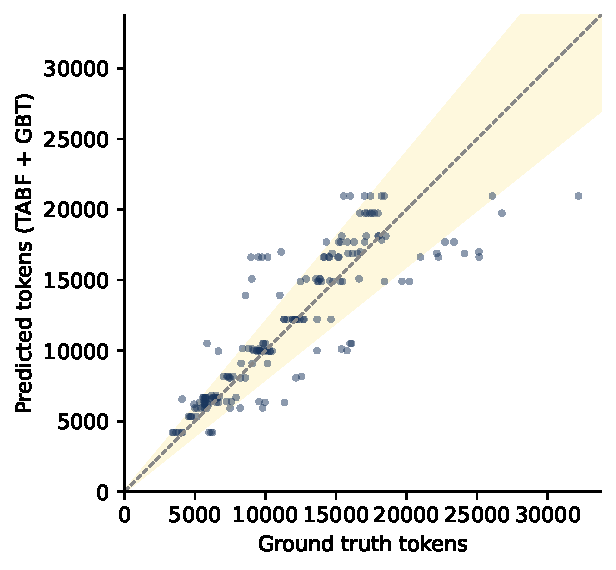
\includegraphics[width=0.45\linewidth]{results/fig_calibration.pdf}
  \hfill
  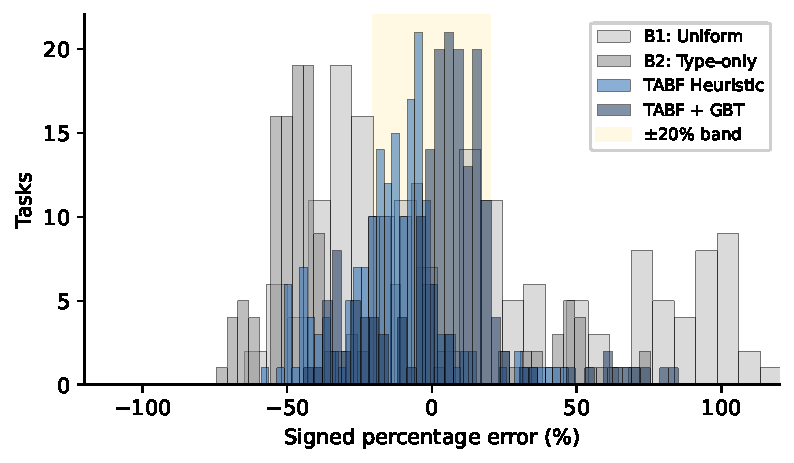
\includegraphics[width=0.50\linewidth]{results/fig_error_dist.pdf}
  \caption{Left: predicted vs.\ ground-truth tokens for TABF\,+\,GBT on
  the test set; the shaded wedge marks the $\pm$20\% band. Right:
  signed percentage-error histograms for four methods. TABF\,+\,GBT's
  distribution is tightly concentrated inside the band, while
  uniform and type-only baselines have heavy tails on both sides.}
  \label{fig:calib}
\end{figure}

\subsection{Per-Task-Type Breakdown}

Table~\ref{tab:stratified} stratifies TABF+GBT errors by latent task
type. Figure~\ref{fig:per_type} ranks task types by within-band rate.

\begin{table}[h]
  \caption{TABF+GBT, stratified by latent task type ($n_\text{test}\,{=}\,185$ tasks total).
  \emph{Avg GT} and \emph{Avg pred} are mean ground-truth and
  predicted tokens respectively.}
  \label{tab:stratified}
  \centering
  \small
  \begin{tabular}{lrrrrrr}
    \toprule
    Task type & $n$ & MAE & MAPE (\%) & W20R (\%) & Avg GT & Avg pred \\
    \midrule
    Bug fix         & 39 & 1{,}147.6 & 10.09 & 87.18 & 11{,}104 & 10{,}960 \\
    Documentation   & 25 &    919.0  & 13.35 & 88.00 &  6{,}417 &  6{,}385 \\
    Data analysis   & 21 & 2{,}159.2 & 14.01 & 80.95 & 15{,}368 & 15{,}355 \\
    Refactoring     & 24 & 1{,}935.5 & 12.50 & 75.00 & 13{,}648 & 13{,}439 \\
    Code generation & 21 &    848.8  & 15.38 & 66.67 &  6{,}683 &  6{,}852 \\
    Research query  & 21 & 2{,}247.8 & 15.27 & 66.67 & 12{,}631 & 13{,}011 \\
    Tool-use chain  & 26 & 3{,}636.4 & 28.54 & 53.85 & 14{,}175 & 15{,}314 \\
    Multi-step plan &  8 & 3{,}635.6 & 29.36 & 50.00 & 12{,}740 & 12{,}197 \\
    \bottomrule
  \end{tabular}
\end{table}

\begin{figure}[!htbp]
  \centering
  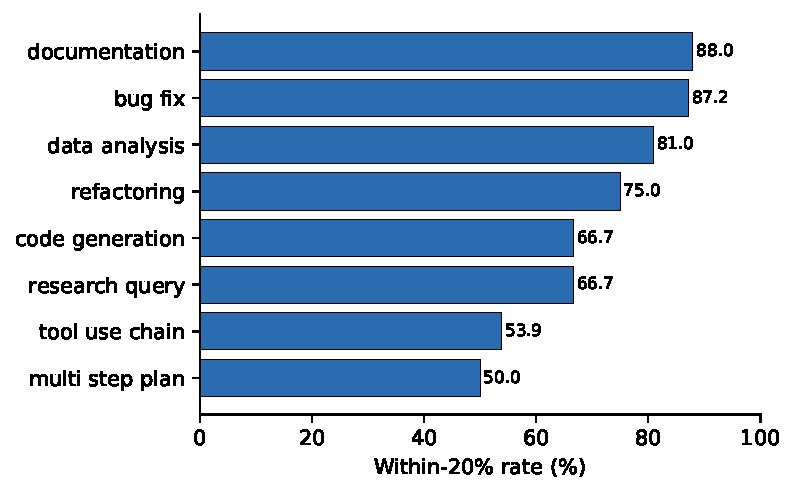
\includegraphics[width=0.62\linewidth]{results/fig_per_type_w20r.pdf}
  \caption{Within-20\% rate per task type for TABF+GBT, sorted.
  Bug fix and documentation are easiest; tool-use chains and
  multi-step plans are hardest (and multi-step plan's sample is also
  the smallest at $n\,{=}\,8$, so its number should be read with
  caution).}
  \label{fig:per_type}
\end{figure}

Tool-use chains and multi-step plans ($n\,{=}\,8$) lag; bug fix and
documentation lead.

\subsection{Ablations}

We ablated the heuristic tier feature-by-feature, dropping one signal
from the pipeline end-to-end (the classifier and forecast both stop
seeing the feature). Table~\ref{tab:ablation} reports the result.

\begin{table}[h]
  \caption{Heuristic ablations. Each row removes one input from the
  pipeline; the full heuristic is the top row. ``No complexity
  scaling'' replaces $\delta(\tau)$ with a constant
  \textsc{medium}.}
  \label{tab:ablation}
  \centering
  \small
  \begin{tabular}{lrrr}
    \toprule
    Configuration & MAE & MAPE (\%) & W20R (\%) \\
    \midrule
    Full TABF heuristic            & 2{,}502.5 & 18.18 & 65.41 \\
    \quad $-$ complexity scaling   & 4{,}769.5 & 35.71 & 30.81 \\
    \quad $-$ \code{has\_code\_keywords}      & 3{,}026.4 & 23.58 & 55.14 \\
    \quad $-$ \code{entity\_count}            & 3{,}085.5 & 22.10 & 57.30 \\
    \quad $-$ \code{has\_multi\_step}         & 2{,}917.6 & 20.39 & 59.46 \\
    \quad $-$ \code{has\_tool\_keywords}      & 2{,}664.0 & 20.10 & 60.54 \\
    \quad $-$ \code{has\_comparison}          & 2{,}760.4 & 19.80 & 62.70 \\
    \quad $-$ \code{has\_file\_refs}          & 2{,}666.6 & 19.26 & 63.24 \\
    \quad $-$ word-count context adjustment   & 2{,}595.5 & 18.81 & 64.86 \\
    \bottomrule
  \end{tabular}
\end{table}

Complexity scaling dominates ($-34.6$~pp W20R when removed); code keywords
and entity count are next.

On the test split, classifier agreement with latent labels is 95.1\%
(task type), 86.5\% (complexity), and 83.2\% (both).

\subsection{Multi-seed cross-validation}
\label{sec:multiseed}

Five-seed CV gives \textbf{71.68 $\pm$ 3.98\%} for TABF\,+\,GBT
(HistGBoost on the same features: 71.46 $\pm$ 3.11\%; full grid in
\code{results/multiseed\_summary.csv}).
TABF\,+\,GBT matches RandomForest/HistGBoost on the same features
(McNemar $p\,{=}\,1.0$); the differentiator is per-stage output and a
no-training heuristic tier.

\subsection{Robustness checks}
\label{sec:robustness}

\paragraph{Per-stage regressors.}
Redistributing a total-token prediction hurt stagewise accuracy (mean
per-stage W20R 53.6\%). Six stage-specific GBT regressors raise mean
per-stage W20R to \textbf{62.9\%} (+9.3~pp) with nearly unchanged total
W20R (73.5\% vs 74.1\%); system-stage W20R rises from 40.5\% to 77.8\%
(Table~\ref{tab:stagewise-gbt}).

\begin{table}[h]
  \caption{Total vs per-stage GBT ($n\,{=}\,185$ synthetic test).}
  \label{tab:stagewise-gbt}
  \centering
  \small
  \begin{tabular}{lrr}
    \toprule
    Model & Total W20R (\%) & Mean stage W20R (\%) \\
    \midrule
    TABF + GBT (redistribute) & 74.05 & 53.60 \\
    TABF + GBT (per-stage)    & 73.51 & \textbf{62.88} \\
    \bottomrule
  \end{tabular}
\end{table}

\paragraph{Real production traces.}
A HistGradientBoosting model trained on 63 of 83 BigQuery agent turns
(task text $\to$ total tokens) reaches \textbf{25.0\%} W20R on the held-out
20 with a train-median scale factor (Table~\ref{tab:real-trace}). Synthetic-only
forecasts without calibration stay near 6\% on the same corpus.

\paragraph{Confidence and stress tests.}
Quantile intervals hit 50\%/75\%/87\% empirical coverage at 50\%/80\%/90\%
nominal levels. Under simulator perturbations (2$\times$ reasoning, shuffled
stage ratios, 2$\times$ noise), learned models hold $\approx$71--74\% W20R
while the heuristic drops to 17\% when ratios are wrong---evidence that
fixed per-stage ratios must be recalibrated per agent.

\begin{table}[!htbp]
  \caption{Oracle vs.\ predicted labels on the synthetic test set ($n\,{=}\,185$).
  Oracle rows use latent type/complexity from the corpus; predicted rows use
  the live classifier (deployment-realistic).}
  \label{tab:oracle-labels}
  \centering
  \small
  \begin{tabular}{lrrr}
    \toprule
    Model & W20R predicted (\%) & W20R oracle (\%) & $\Delta$ (pp) \\
    \midrule
    TABF heuristic & 63.2 & 74.1 & +10.8 \\
    TABF + GBT     & 71.4 & 73.5 & +2.2 \\
    \bottomrule
  \end{tabular}
\end{table}

\begin{table}[!htbp]
  \caption{Forecasting on real BigQuery agent turns.}
  \label{tab:real-trace}
  \centering
  \small
  \begin{tabular}{lrrl}
    \toprule
    Setting & $n_\text{test}$ & W20R (\%) & Calibration \\
    \midrule
    Trained on 63 real turns      & 20 & 25.0 & train-median scale \\
    LOO on 83 turns               & 83 & 15.7 & LOO-median scale \\
    Synthetic TABF+GBT, no scale  & 83 &  6.0 & none \\
    \bottomrule
  \end{tabular}
\end{table}

\section{Complementary In-Loop Optimisation: ContextOptimizer}
\label{sec:optimizer}

TABF's 26\% forecast tail and runtime drift from large tool results and
growing memory motivate a complementary in-loop pipeline,
ContextOptimizer, that runs immediately before every LLM call
and trims the live message list to fit the budget. The optimiser is
framework-agnostic, pure-stdlib in its default configuration (no LLM
call inside the optimiser itself), and ships with two invariants so it
can drop into any tool-using agent without breaking the OpenAI API
contract.

\subsection{The funnel: four layer categories}

The pipeline composes a fixed sequence of layer categories
(Figure~\ref{fig:funnel}). Each \emph{layer} is a pure function from a
list of canonical \code{ContextItem}s to a (typically shorter) list.

\begin{figure}[!htbp]
  \centering
  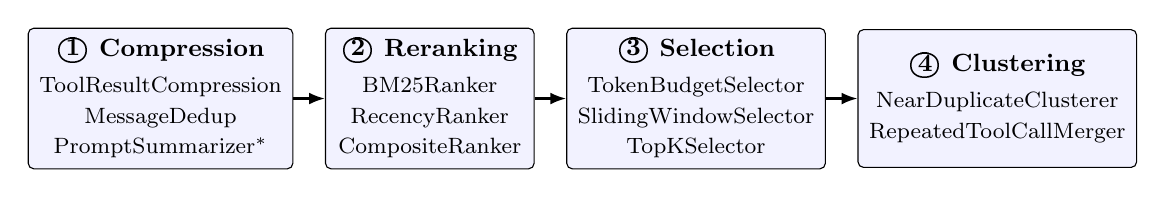
\begin{tikzpicture}[
    node distance=0.6cm and 0.4cm,
    box/.style={draw, rounded corners=2pt, align=center, minimum width=2.65cm,
                minimum height=1.75cm, font=\small, inner sep=4pt},
    arrow/.style={-{Latex[length=2mm]}, thick}
  ]
    \node[box, fill=blue!5] (s1) {\textbf{\textcircled{1} Compression}\\[2pt]
      \footnotesize ToolResultCompression\\\footnotesize MessageDedup\\\footnotesize PromptSummarizer$^*$};
    \node[box, fill=blue!5, right=of s1] (s2) {\textbf{\textcircled{2} Reranking}\\[2pt]
      \footnotesize BM25Ranker\\\footnotesize RecencyRanker\\\footnotesize CompositeRanker};
    \node[box, fill=blue!5, right=of s2] (s3) {\textbf{\textcircled{3} Selection}\\[2pt]
      \footnotesize TokenBudgetSelector\\\footnotesize SlidingWindowSelector\\\footnotesize TopKSelector};
    \node[box, fill=blue!5, right=of s3] (s4) {\textbf{\textcircled{4} Clustering}\\[2pt]
      \footnotesize NearDuplicateClusterer\\\footnotesize RepeatedToolCallMerger};
    \draw[arrow] (s1) -- (s2);
    \draw[arrow] (s2) -- (s3);
    \draw[arrow] (s3) -- (s4);
  \end{tikzpicture}
  \caption{The ContextOptimizer funnel. Compression squeezes content
  inside individual items, reranking scores items by relevance,
  selection picks which items to keep within the token budget, and
  clustering merges near-duplicates. The starred summariser is the only
  layer that can optionally invoke an LLM and is off in the default
  configuration.}
  \label{fig:funnel}
\end{figure}

\subsection{Canonical message type and adapters}

Every layer operates on a single canonical type, \code{ContextItem}, with
fields \code{role}, \code{content}, \code{name}, \code{tool\_call\_id},
\code{tool\_calls}, \code{pinned}, and \code{meta}. Concrete agent
frameworks plug in through a thin \code{Adapter} protocol:

\begin{itemize}\setlength{\itemsep}{0pt}
  \item \code{LangChainAdapter} round-trips \code{SystemMessage},
        \code{HumanMessage}, \code{AIMessage}, and \code{ToolMessage}.
  \item \code{OpenAIAdapter} round-trips the OpenAI Chat-Completions
        message dict shape.
  \item \code{GenericAdapter} round-trips plain
        $\{\code{role},\ \code{content}\}$ dictionaries.
\end{itemize}

Adding support for a new framework is a single class implementing two
methods (\code{to\_items} and \code{from\_items}). The reference
implementation is 22 lines for the \code{Adapter} protocol plus
${\sim}100$~lines for each concrete adapter; the entire optimiser
package is ${\sim}2{,}000$ lines of Python including docstrings.

\subsection{Invariant preservation}
\label{sec:invariants}

An aggressive trimmer that produces a message list the LLM rejects is
worse than no trimmer at all: the request returns a 400 and the user
sees a stack trace instead of an answer. The pipeline therefore
treats two properties as hard invariants, enforced after every layer
runs rather than relied on as politeness from each layer:

\begin{enumerate}\setlength{\itemsep}{0pt}
  \item \textbf{Pinned items survive.} Items marked \code{pinned=True}
        (typically the system prompt and the current user message) are
        never dropped, regardless of token budget.
  \item \textbf{Tool-call/response pairing.} If an assistant message
        carries a \code{tool\_calls} block, every referenced
        \code{tool\_call\_id} must be matched by a subsequent
        \code{role="tool"} response, in original order. The pipeline
        repairs accidental splits using stable positional metadata
        (\code{\_ctxopt\_pos}) written when items first enter the
        pipeline.
\end{enumerate}

Orphan \code{tool\_call\_id}s after aggressive dedup caused OpenAI 400s;
pairing is therefore a pipeline invariant, not a per-layer concern.

\subsection{Three presets}

Most teams will pick one of three presets rather than compose layers by
hand. Table~\ref{tab:presets} summarises them.

\begin{table}[h]
  \caption{The three ContextOptimizer presets. \code{LLM?} indicates
  whether the optimiser itself makes an LLM call (the summariser layer
  is optional and off by default in \emph{aggressive}). \emph{Typical
  use} is the deployment scenario each preset is calibrated for.}
  \label{tab:presets}
  \centering
  \footnotesize
  \begin{tabular}{lllll}
    \toprule
    Preset & Layers & Max tokens & LLM? & Typical use \\
    \midrule
    \emph{Minimal}    & Compression + SlidingWindow                    & 8{,}000 & No   & Short chat, smoke tests \\
    \emph{Balanced}   & Compression + BM25/Recency + TokenBudget       & 8{,}000 & No   & Default production \\
    \emph{Aggressive} & Full funnel + clusterer (+ summariser$^*$)     & 4{,}000 & Opt. & Long multi-turn \\
    \bottomrule
  \end{tabular}
\end{table}

\paragraph{Pairing with TABF.}
\label{sec:pairing}

TABF can set ContextOptimizer's \code{max\_tokens} at dispatch; the
pairing is not live yet. Production today uses a fixed budget;
Table~\ref{tab:real-trace} shows that models trained on local traffic
(63 train / 20 test) outperform synthetic-only transfer. A one-time
median scale fit on the first ${\sim}100$ turns is the recommended
deployment step.

\section{Production Deployment Case Study}
\label{sec:production}

ContextOptimizer runs in production on a LangGraph NL-to-SQL agent over
BigQuery (TABF is offline; Section~\ref{sec:pairing}). Numbers come from
14 ctx-opt log lines (72\% savings), 83 turns of BigQuery eval telemetry,
and a 100-run in-container microbench; released CSVs live in
\mbox{\texttt{results/}}.
Figure~\ref{fig:prod-stack} sketches the deployment: Chainlit
$\to$ GraphQL/Starlette $\to$ LangGraph $\to$ ContextOptimizer
(balanced preset) $\to$ \code{gpt-4o-mini}, with Spanner checkpoints,
Langfuse traces, and a six-table BigQuery eval pipeline as observability
fan-outs.

\begin{figure}[H]
  \centering
  \resizebox{\linewidth}{!}{%
  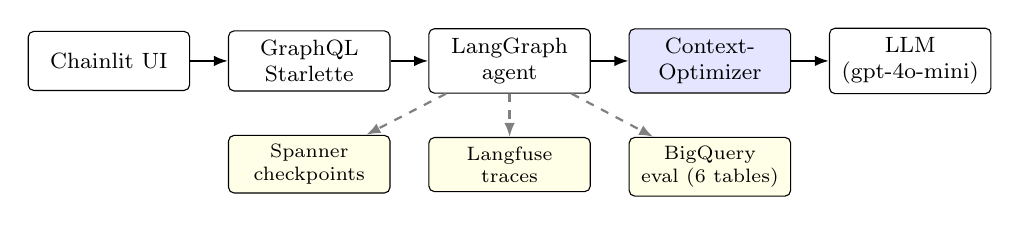
\begin{tikzpicture}[
    node distance=0.38cm and 0.48cm,
    box/.style={draw, rounded corners=2pt, align=center, font=\footnotesize,
                minimum width=2.05cm, minimum height=0.75cm},
    obs/.style={draw, rounded corners=2pt, align=center, font=\scriptsize,
                fill=yellow!10, minimum width=2.05cm, minimum height=0.62cm},
    arrow/.style={-{Latex[length=1.8mm]}, thick}
  ]
    \node[box] (ui) {Chainlit UI};
    \node[box, right=of ui] (gql) {GraphQL\\Starlette};
    \node[box, right=of gql] (lg) {LangGraph\\agent};
    \node[box, fill=blue!10, right=of lg] (co) {Context-\\Optimizer};
    \node[box, right=of co] (llm) {LLM\\(gpt-4o-mini)};

    \draw[arrow] (ui) -- (gql);
    \draw[arrow] (gql) -- (lg);
    \draw[arrow] (lg) -- (co);
    \draw[arrow] (co) -- (llm);

    \node[obs, below=0.55cm of gql] (sp) {Spanner\\checkpoints};
    \node[obs, below=0.55cm of lg] (lf) {Langfuse\\traces};
    \node[obs, below=0.55cm of co] (bq) {BigQuery\\eval (6 tables)};

    \draw[arrow, dashed, gray] (lg) -- (sp);
    \draw[arrow, dashed, gray] (lg) -- (lf);
    \draw[arrow, dashed, gray] (lg) -- (bq);
  \end{tikzpicture}%
  }
  \caption{Production deployment. Yellow boxes are observability
  fan-outs; the dashed arrows are asynchronous writes.}
  \label{fig:prod-stack}
\end{figure}

\paragraph{Per-call token savings.}
Table~\ref{tab:prod-savings} aggregates 14 LLM calls captured from
interactive sessions over a 24-hour window. Of the 14 calls, 12
engaged the optimiser (the conversation history had at least one
compressible tool result), 2 were no-ops (the optimiser ran but had
nothing to trim), and 0 grew. The aggregate input-token reduction is
72.0\% (74.0\% on calls that engaged), with the tightest single call
compressing 14{,}949 tokens down to 1{,}828
(ratio~0.12). Figure~\ref{fig:prod-savings} plots four real per-call
log lines plus the aggregate.

\begin{table}[H]
  \caption{Aggregate input-token savings across 14 directly-captured
  production optimiser log lines (balanced preset). \emph{No-op} means
  the optimiser ran but had no work to do. Source:
  \code{results/production\_token\_savings\_summary.csv}.}
  \label{tab:prod-savings}
  \centering
  \small
  \begin{tabular}{lr}
    \toprule
    Metric & Value \\
    \midrule
    LLM calls observed                          & 14 (12 saved, 2 no-op, 0 grew) \\
    Tokens sent without optimiser               & 215{,}438 \\
    Tokens sent with optimiser                  & 60{,}250 \\
    \textbf{Tokens saved}                       & \textbf{155{,}188} \\
    \textbf{Reduction (overall)}                & \textbf{72.0\%} \\
    Reduction (engaged calls only)              & 74.0\% \\
    Best single-call compression ratio          & 0.12 (14{,}949 to 1{,}828 tokens) \\
    \bottomrule
  \end{tabular}
\end{table}

\begin{figure}[H]
  \centering
  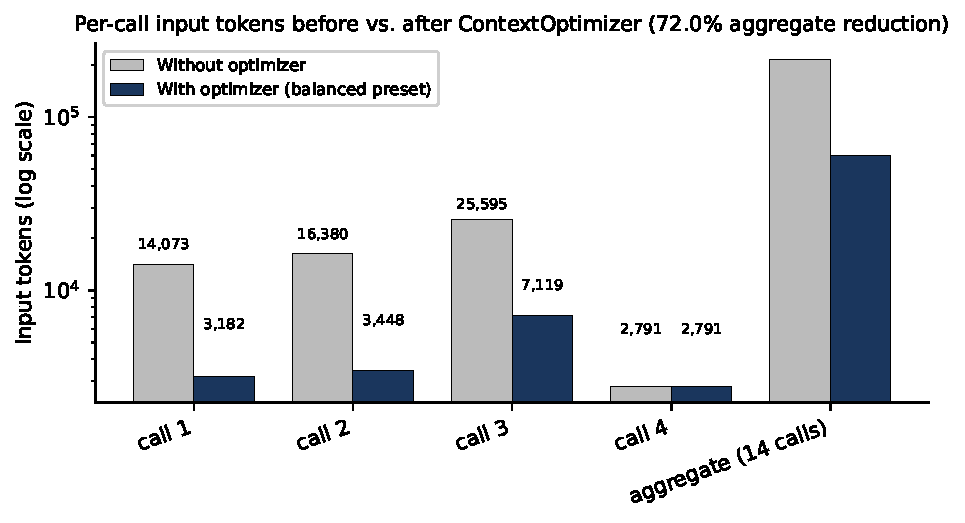
\includegraphics[width=0.72\linewidth]{results/fig_production_savings.pdf}
  \caption{Per-call input tokens before vs.\ after ContextOptimizer.
  Four real per-call log lines (left) plus the aggregate over all 14
  calls (right). The log y-axis makes both ends of the distribution
  visible; the no-op call is intentionally untouched to illustrate the
  invariant-preservation behaviour. The 4-row sample CSV is released as
  \code{results/production\_token\_savings\_samples.csv}.}
  \label{fig:prod-savings}
\end{figure}

\paragraph{Annualised cost projections.}
Projected savings multiply the 83-turn mean input (27{,}757 tokens) by the
72\% reduction from 14 observed calls (${\approx}$20K tokens saved per
turn). Table~\ref{tab:prod-cost} and Figure~\ref{fig:prod-cost} apply
that to three public list prices (input tokens only, 2026-05-20).

\begin{table}[H]
  \caption{Projected USD savings from ContextOptimizer at three model
  price points. \emph{Derivation:} avg input tokens per turn
  (27{,}757; n=83 production turns) $\times$ measured 72\% reduction
  $=$ 19{,}985 saved input tokens per turn. Public list prices captured
  2026-05-20. Input tokens only. Source:
  \code{results/production\_cost\_projections.csv}.}
  \label{tab:prod-cost}
  \centering
  \small
  \begin{tabular}{lrrrrr}
    \toprule
    Model & per turn & 100/day & 1k/day & 10k/day & \textbf{Annual @ 1k/day} \\
    \midrule
    \code{gpt-4o-mini}        & \$0.0030 & \$0.30  & \$3.00   & \$29.98   & \textbf{\$1{,}094} \\
    \code{gpt-4o}             & \$0.0500 & \$5.00  & \$49.96  & \$499.62  & \textbf{\$18{,}236} \\
    \code{claude-sonnet-4.5}  & \$0.0600 & \$6.00  & \$59.95  & \$599.55  & \textbf{\$21{,}883} \\
    \bottomrule
  \end{tabular}
\end{table}

\begin{figure}[H]
  \centering
  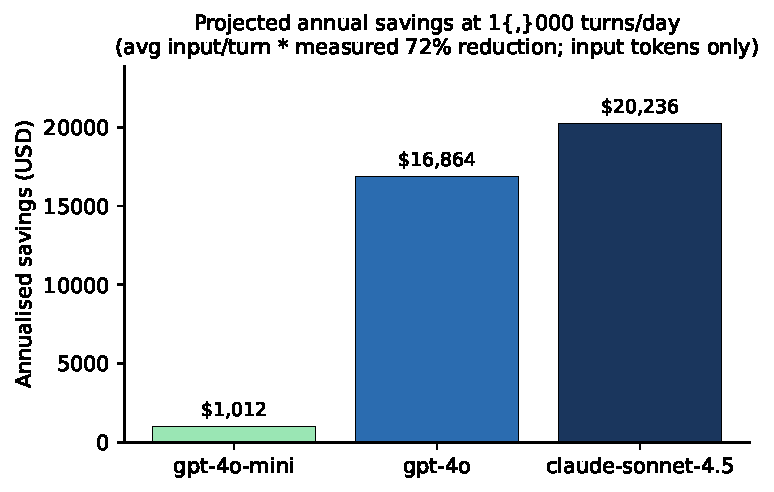
\includegraphics[width=0.55\linewidth]{results/fig_production_costs.pdf}
  \caption{Annualised savings at 1{,}000 turns/day across three model
  price points. The gap between \code{gpt-4o-mini} and \code{gpt-4o}
  is $\approx\!17\times$, mirroring the published list-price ratio.}
  \label{fig:prod-cost}
\end{figure}

\paragraph{Trajectory and quality on production turns.}
Table~\ref{tab:prod-bq-pop} summarises the 83-turn population;
Table~\ref{tab:prod-quality} joins the same \code{request\_id}s to
\code{agent\_quality\_eval} (task-success proxy and latency).

\begin{table}[h]
  \caption{Per-turn distribution from the production BigQuery
  agent-eval pipeline. \emph{N} is the number of turns each metric is
  computed over (different metrics are populated by different
  pipeline writers, so the populations differ slightly). Source:
  \code{results/production\_bq\_population\_stats.csv}.}
  \label{tab:prod-bq-pop}
  \centering
  \small
  \begin{tabular}{lrrrrr}
    \toprule
    Metric & $N$ & Mean & Median & p95 & Max \\
    \midrule
    LLM calls per turn       & 83  &  6.47    & 6      & 14     & 22     \\
    Input tokens per turn    & 83  & 27{,}757 & 22{,}382 & 64{,}922 & 90{,}637 \\
    Trajectory steps / turn  & 128 &  8.35    & 6      & 20     & 34     \\
    Tool calls per turn$^{\dagger}$ & 123 &  2.82 & 2 & 7 & 12 \\
    \bottomrule
  \end{tabular}\\[2pt]
  {\footnotesize $^{\dagger}$Counted on turns with at least one tool
  invocation; turns with zero tool calls are excluded from this row only.}
\end{table}

\begin{table}[h]
  \caption{Downstream outcomes on the same 83 production turns
  (\code{agent\_quality\_eval}). We do not have a no-optimiser A/B;
  these are observational baselines.}
  \label{tab:prod-quality}
  \centering
  \small
  \begin{tabular}{lr}
    \toprule
    Metric & Value \\
    \midrule
    Turns with eval row                     & 83 \\
    Status \code{complete} (proxy success)  & 77.1\% \\
    Median latency, complete turns          & 26.5\,s \\
    Median latency, \code{error} turns      & 8.6\,s \\
    Median input tokens, complete           & 22{,}530 \\
    \bottomrule
  \end{tabular}
\end{table}

\paragraph{Optimiser overhead (microbench).}
\label{sec:microbench}

Overhead figures (Table~\ref{tab:prod-overhead}) come from the
microbenchmark, not the 14 production log lines, which did not record
per-call wall clock. The 14 production log lines also do not record
\emph{which} layer was responsible for the saved tokens.
We therefore ran a 100-call microbenchmark of the \code{balanced}
preset inside the production container, against synthetic-but-
production-shaped inputs that bracket the 83-turn input distribution
(1.6K to 449K input tokens; 5 repeats over a 20-cell grid of
\code{tool\_calls} $\times$ \code{rows\_per\_tool\_call}). The
microbenchmark script and the two output CSVs
(\code{optimizer\_microbench.csv}, \code{optimizer\_microbench\_layers.csv})
are released with the paper.

Table~\ref{tab:prod-overhead} reports the per-call overhead
distribution. The mean of 99~ms is dominated by the largest inputs in
the grid (the p95 of 529~ms corresponds to the 449K-token 8-tool
scenario, which is well above the p95 production turn of 65K~tokens).
The median of 48~ms is closer to the production-median input size and
is the more representative number for a typical call.

\begin{table}[h]
  \caption{Per-call wall-clock overhead of the \code{balanced} preset
  (100 runs, synthetic production-shaped inputs).
  Source: \code{results/optimizer\_microbench.csv}.}
  \label{tab:prod-overhead}
  \centering
  \small
  \begin{tabular}{lr}
    \toprule
    Statistic & ms \\
    \midrule
    Mean              &  99.29 \\
    Median            &  48.52 \\
    p95               & 529.05 \\
    Max               & 535.93 \\
    \bottomrule
  \end{tabular}
\end{table}

On synthetic production-shaped inputs, tool-result compression accounts
for all measured savings; median overhead is 49\,ms (p95 529\,ms on
449K-token stress cells). See \code{results/optimizer\_microbench*.csv}.

\subsection{Generic-agent personas and compression baseline}
\label{sec:personas}

Four synthetic personas (ReAct search, code-fix with duplicate reads,
multi-turn RAG, status polling; 25 seeds each) exercise different
funnel layers. Table~\ref{tab:personas} reports ContextOptimizer;
Table~\ref{tab:compress-baseline} adds a training-free baseline (B9:
head-tail tool truncation plus middle-history drop to 8K tokens).

\begin{table}[h]
\centering
\caption{Per-persona ContextOptimizer results, balanced preset,
gpt-4o-mini token counter, 25 seeds each. Sources:
\code{results/generic\_agents.csv} (totals) and
\code{results/generic\_agents\_layers.csv} (layer attribution).}
\label{tab:personas}
\small
\begin{tabular}{l r r r r r}
\toprule
Persona & Tokens before & Tokens after & Reduction & Ratio & Wall-clock \\
        & (mean / run) & (mean / run) & (\%)       &       & (ms / run) \\
\midrule
ReAct web search       & 1{,}977  & 1{,}033 & 47.7\% & 0.523 & 20.1 \\
Code-fix               & 7{,}975  & 678     & 91.5\% & 0.085 & 11.3 \\
Multi-turn research    & 16{,}777 & 6{,}320 & 62.3\% & 0.377 & 30.9 \\
Polling                & 907      & 260     & 71.3\% & 0.287 & 1.9 \\
\midrule
Overall (100 runs)     & 6{,}909  & 2{,}073 & 70.0\% & 0.300 & 16.1 \\
\bottomrule
\end{tabular}
\end{table}

\begin{figure}[!htbp]
\centering
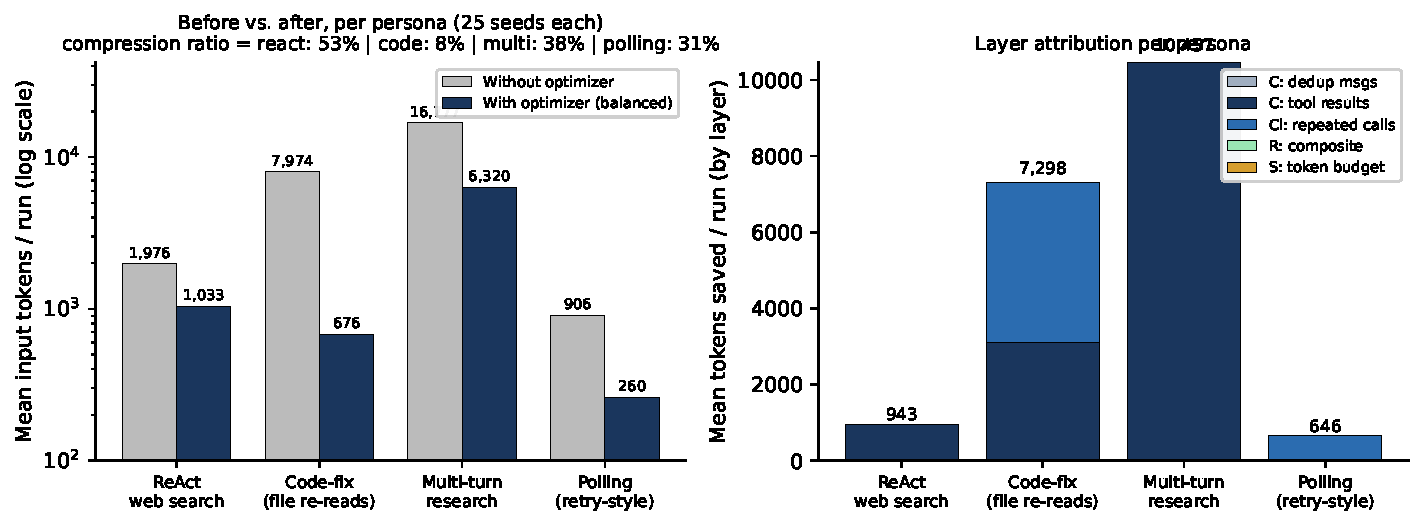
\includegraphics[width=0.92\linewidth]{results/fig_generic_agents.pdf}
\caption{Persona benchmark: tokens before/after (left) and per-layer
savings (right), balanced preset, 25 seeds each.}
\label{fig:personas}
\end{figure}

\begin{table}[H]
  \caption{Training-free truncation baseline (B9) vs ContextOptimizer,
  mean input-token reduction (\%), 25 seeds per persona.}
  \label{tab:compress-baseline}
  \centering
  \small
  \begin{tabular}{lrr}
    \toprule
    Persona & B9 truncate & ContextOptimizer \\
    \midrule
    ReAct web search    & 42.2 & 47.7 \\
    Code-fix            &  3.5 & 91.5 \\
    Multi-turn research & 92.9 & 62.3 \\
    Polling             &  0.0 & 71.3 \\
    \bottomrule
  \end{tabular}
\end{table}

ContextOptimizer wins on duplicate reads and polling where dedup and
clustering engage; naive truncation overshoots on long RAG history.
Fixtures are synthetic; a second live deployment remains future work.

\FloatBarrier
\section{Discussion and limitations}
\label{sec:discussion}

\paragraph{Composition.}
TABF (pre-flight) and ContextOptimizer (in-loop) are designed to compose
but are not wired end-to-end in production: the optimiser still uses a
static \code{max\_tokens}. Offline replay and real-trace training
(Section~\ref{sec:robustness}) show that forecasts need a per-deployment
scale factor or retraining on ${\sim}100$ local turns before they gate
budgets reliably.

\paragraph{Forecasting.}
The synthetic corpus shares features with TABF's classifier
(Section~\ref{sec:setup}); oracle-label analysis (Table~\ref{tab:oracle-labels})
shows limited inflation for GBT ($+$2.2~pp) but larger inflation for the
heuristic ($+$10.8~pp). GBT matches RandomForest/HistGBoost on the same
hand features; TF-IDF baselines (64--70\% W20R) bound what raw text alone
achieves without task-type rules. We have no cross-domain or cross-model
generalisation study; English keyword rules and eight lexical features may
fail on multilingual or domain jargon. Real traces: ${\approx}$6\% W20R
without calibration, 25\% with 63/20 train/test on one BigQuery agent---not
yet strong enough for unattended budget gating.

\paragraph{Optimisation.}
Evidence is small and observational: 14 instrumented calls (72\% savings),
83-turn telemetry, no randomised quality A/B vs.\ an unoptimised control.
Persona and B9 truncation baselines (Table~\ref{tab:compress-baseline}) are
synthetic; CompactPrompt-style compression on live multi-turn logs and Tool
Attention-style schema gating in production are not yet measured. A unified
TABF$\to$ContextOptimizer dispatch path (forecast sets \code{max\_tokens},
logs $(\text{forecast},\text{realised},\text{saved})$ for retraining) is
designed but not deployed.

\section{Conclusion}
\label{sec:conclusion}

Token budgeting in agentic LLM workflows can be addressed before the
agent runs and during the agent's loop, and neither side needs to be
expensive. Pre-flight, a small pipeline of eight lexical features, a
rule-based classifier, a lookup table, and an optional 120-tree GBT
places 74\% of forecasts inside a $\pm 20\%$ band on a 600-task
benchmark, with no LLM call and millisecond-level overhead. In-loop,
a four-layer trimming pipeline (ContextOptimizer) cut input-token
consumption by 72\% across 14 directly-observed LLM calls in one
production deployment (a LangGraph NL-to-SQL agent over BigQuery)
while preserving tool-call/response pairing as a hard invariant,
and engaged a different combination of layers on each of four
additional agent personas evaluated synthetically. The product of that 72\% reduction and
the measured per-turn input of 27{,}757 tokens (83-turn population)
gives per-turn savings of roughly 20{,}000 tokens, which at 1{,}000
turns per day is \$1{,}094 per year on \code{gpt-4o-mini},
\$18{,}236 on \code{gpt-4o}, and \$21{,}883 on \code{claude-sonnet-4.5}.
The two stages are designed to compose: the forecast sets a target and
the optimiser enforces it. Real-trace training and per-stage GBT regressors address the largest
forecasting gaps; production still needs dispatcher wiring and a quality
A/B. The implementations of both frameworks, the synthetic benchmark,
the production CSVs, the 100-run microbenchmark, and all seeds are
released with this paper.

\FloatBarrier
\bibliographystyle{plainnat}
\bibliography{paper}

\end{document}
